% Section 6 -- Capstone validation (manuscript.md lines 357-492).
% Numbers, verdicts, and Korean frozen sentences are copied verbatim from
% the manuscript; see ../CONVERSION.md for the binding rules.

\section{Capstone validation: finite-density detectability of the conformal class}
\label{sec:capstone}

The ladder reconstructs quantities from supplied ingredients inside flat
models; \sref{sec:negative} bounds it from below. This section caps it from
the other side, with the converse of the first negative result.
\Sref{sec:r5} showed that \emph{within} a conformal class, order carries no
scale: positive rescalings leave the causal matrix unchanged. By the theorems
that motivate the program, order determines the conformal class itself---so
\emph{across} conformal classes order must differ. Whether that difference
survives finite density, for a curvature channel that touches nothing but the
order, is the question this capstone answers affirmatively, as a
preregistered experiment (P14 in the program's internal numbering; within
this program, the first finite-density crossing of the conformal-flatness
ceiling, via a 4D type~N pure-Weyl construction).

\subsection{The \texorpdfstring{$(1{+}1)$D}{(1+1)D} conformal ceiling}
\label{sec:ceiling}

Every $(1{+}1)$D metric is conformally flat, so in the $(1{+}1)$D stages of
this program (and its curvature-focused companions P12--P13) curvature could
reach the order only through the volume-coefficient channel: those
experiments tested curvature entering through the measure/counting channel,
and the channel in which order directly carries a conformal-class difference
could not be tested there at all. This was an intended dimensional limit of
the models, not a confounded experiment: Weyl curvature---the conformal-class
content of curvature---is identically zero below four spacetime dimensions,
so a direct test needs a 4D construction built so that the measure channel is
exactly frozen while the conformal class moves.

\subsection{Pure-Weyl control construction}
\label{sec:pureweyl}

The construction is a vacuum plane wave in Brinkmann coordinates with profile
$A(u)(x^2 - y^2)$ on a constant-$A$ slab: Ricci-flat, Petrov type~N, with
$\det g = -1$ identically. Because $\det g = -1$, the coordinate volume form
and the Poisson sprinkling law are \emph{identical} to flat spacetime. That
identity supports the strongest form of pairing, and \emph{C1 uses it}: C1's
control reading is the \emph{same sprinkled point set} read with $A = 0$, so
for C1 any difference between the two readings is a functional of the
relation change alone---it cannot be a sampling artifact, an intensity
mismatch, or a calibration residual. C2 deliberately does \emph{not} pair:
its two arms are independent, unpaired sprinkling streams drawn under the
identical sprinkling law, with finite-sample variation controlled by its
frozen interval rules rather than removed by pairing---because its claim is
about telling one ensemble's posets from the other's, not about a
within-point-set counterfactual (\sref{sec:design}). What is \emph{not}
identical between geometries is the causal-diamond volume: the light-cone
boundary tilts, and at equal proper time the curved-arm diamond volume sits
0.4\% ($wT = 1$) to 7.3\% ($wT = 2$) above flat---a deterministic design
check pins both numbers, against the closed form
$V_A/V_0 = 1 + (wT)^4/252 + O((wT)^8)$. Those percentages describe a small
diamond on the axis, and the frozen operating point is neither small nor
on-axis: the probe chain selected \artifact{aniso-a1.0}, a slab spanning
$1/\pi = 0.318$ of the way to the first conjugate point, on a box elongated
three to one along the focusing transverse axis. The order statistic
therefore reads mostly off-axis pairs in the direction where the cones open,
which is why its response is a factor of three rather than a few percent.
This is a deliberately strong operating point, not a weak-curvature probe.
``Same measure'' here means the volume form and
sprinkling law only, never interval volumes; conflating the two was the first
design draft's central error, caught in review, and the distinction is
load-bearing.

\subsection{Finite-density detection design}
\label{sec:design}

An exploratory probe chain (four probes and a confirmation stage, run on seed
streams disjoint from everything that follows) selected the operating
point---slab $(1.0, 1.0, 2.0, 6.0)$, $w = 1.0$, expected 300 events per
sprinkling---and the primary statistic, the global relation fraction (the one
candidate computable from a single poset alone). The preregistered stage then
froze two claims with deliberately different boundaries, never merged into
one sentence:
\begin{itemize}
\item \textbf{C1 (paired ensemble mean).} The estimand is
  $\theta_\Delta = E[f_A - f_0]$, the ensemble mean of the \emph{net} change
  of the relation fraction over paired readings of the same points---not any
  single point set's displacement, and not the gained-plus-lost total motion.
  Confirmation requires the 95\% Student-$t$ interval of the mean paired
  difference ($n = 3000$ sprinklings) to sit entirely above a frozen margin
  $\varepsilon_\Delta = 3.579\times10^{-4}$, an operational margin anchored
  to the probe chain's confirmed block.
\item \textbf{C2 (single-poset classifier, independent replication).} A
  frozen classifier reading only the single-poset relation fraction must
  separate curved from flat ensembles ($n = 4800$ per unpaired arm) under
  three frozen interval rules (standardized separation, AUC with an exact
  boundary bound at complete separation, balanced accuracy), each with its
  own equivalence band. This claim replicates the probe chain's confirmation
  stage on fresh seeds; its failure would have been reported as a conflicting
  replication, never a retroactive cancellation.
\end{itemize}

The stage verdict POSITIVE requires both claims confirmed, certified as a
joint event before execution (4000/4000 joint-effect replicates; the null
branches certify each claim's equivalence power separately at an exact
Clopper--Pearson~\cite{clopperpearson1934} 95\% lower bound of at least 0.90; a joint equivalence
verdict is deliberately not defined, because its joint null rate sits below
that floor at the frozen sizes).

\subsection{Preregistered result}
\label{sec:preregresult}

The campaign ran once, from a clean checkout of the freeze commit, on frozen
seeds, and recorded the executing commit in the artifact. Both claims
confirmed; the stage is POSITIVE (\tref{tab:capstone}).
\Fref{fig:capstone} shows both claims.

\begin{table}[t]
\caption{Preregistered capstone verdicts. Both claims confirmed; the stage
is POSITIVE.}
\label{tab:capstone}
\centering
\begin{tabularx}{\textwidth}{@{}>{\raggedright\arraybackslash}p{9.5pc}l>{\raggedright\arraybackslash}X@{}}
\toprule
Claim & Verdict & Result (95\% CI) \\
\midrule
C1 paired ensemble mean, $n = 3000$ & confirmed &
  mean 0.0502929 $[0.0501046, 0.0504812]$; lower end $140\times$ the margin
  $3.579\times10^{-4}$ \\
C2 classifier replication, $n = 4800$/arm & confirmed &
  separation $s = 11.198$ $[11.035, 11.362]$; AUC $= 1.0$
  $[0.999232, 1.0]$; balanced accuracy $= 1.0$ $[0.986, 1.014]$ \\
\bottomrule
\end{tabularx}
\end{table}

\begin{figure}[t]
\centering
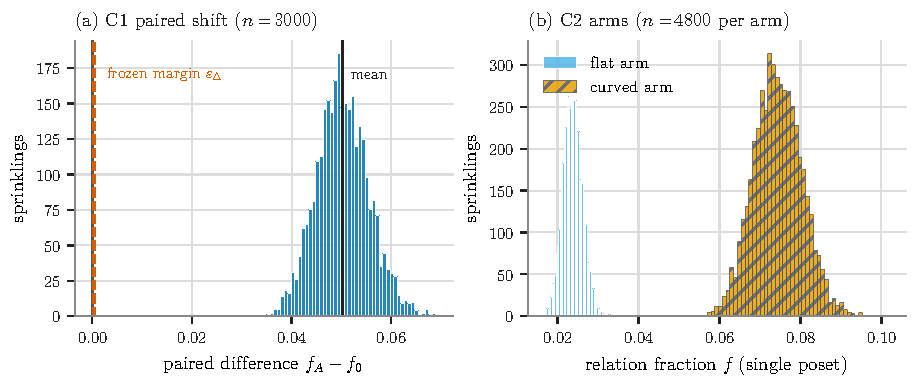
\includegraphics[width=0.95\textwidth]{figures/fig4_capstone.pdf}
\caption{(a) The distribution of the paired per-sprinkling relation-fraction
differences $f_A - f_0$ ($n = 3000$), with mean 0.0502929 (95\% CI
$[0.0501046, 0.0504812]$); the CI lower end is $140\times$ the frozen
margin $\varepsilon_\Delta = 3.579\times10^{-4}$ (marked); (b) the single-poset
relation-fraction samples of the two unpaired arms ($n = 4800$ per arm),
which are completely separated (the frozen exact-bound AUC interval is
$[0.999232, 1.0]$). Both panels are drawn from the committed artifact
(\artifact{docs/\allowbreak{}prereg/\allowbreak{}p14\_\allowbreak{}prereg\_\allowbreak{}results.json}); no value is typed in.}
\label{fig:capstone}
\end{figure}

The size of the effect is worth stating in the statistic's own units, which
the margin ratio hides: averaged over the paired readings the relation
fraction runs 0.023830 flat against 0.074123 curved, a factor of 3.11. The
two arms' relation-fraction samples are completely separated (the minimum
curved-arm value exceeds the maximum flat-arm value in 4800 draws per arm);
the AUC interval at complete separation is the frozen exact bound, not the
degenerate Wald interval. The balanced-accuracy interval got no such
treatment: its frozen construction is an unclipped Wald interval on a
worst-case standard error, so at BA $= 1.0$ it reaches 1.014, outside the
range the quantity can take. That is what the preregistration licenses and it
is printed as it stands; no verdict depends on it, because the gate reads only
the lower end. For the reader's orientation---not as a re-scored gate---the
construction the later S5 stage uses for the same quantity, a
Clopper--Pearson interval per arm combined across the two, gives
$[0.998176, 1.0]$ on the same test halves. Every relation census in both
claims recorded zero
ambiguous and zero escalated pairs. The two sentences the stage licenses were
fixed in the preregistration before execution and are recorded in the
artifact; in translation they are C1, \emph{the paired ensemble mean shift
exceeds $\varepsilon_\Delta$}, and C2, \emph{the probe chain's separation is
independently reproduced}
(\artifact{docs/\allowbreak{}prereg/\allowbreak{}p14\_\allowbreak{}prereg\_\allowbreak{}results.json};
appendix~\ref{app:provenance} records the language of the frozen originals
and what holds these renderings to them).

\subsection{What this establishes}
\label{sec:establishes}

At a fixed box, density, and profile, an order-only statistic separates flat
from curved ensembles: the conformal-class information that order carries by
theorem is \emph{present in the order at finite density}, in the one
construction where the sprinkling measure is exactly frozen. The claim is
existence, not sensitivity. No density or amplitude sweep was run, so nothing
here locates the point at which the separation would fail, and the operating
point was chosen to be strong (\sref{sec:pureweyl}) rather than marginal.
Together with \sref{sec:r5} this
closes the conformal story in both directions---within a class, order is
blind to scale; across classes, at least at this operating point, order
visibly moves.

\subsection{What the plane-wave result alone does not establish}
\label{sec:notestablish}

It says nothing about sensitivity. The frozen operating point was chosen to
be strong, and two things follow that the stage cannot answer: no density or
amplitude sweep was run, so the density at which the separation fails is
unmeasured; and the slab is elongated three to one along the focusing
transverse axis, so whether the effect survives at an isotropic box is
untested. Beyond that, it is not a general-Weyl discriminator (the plane wave
is Petrov type~N and its exact volume form is unrepresentative); it is not
Weyl-tensor recovery
(detection and recovery are different claims; no reconstructed quantity is
produced, which is why this is a capstone boundary experiment and not a new
ladder rung); it does not establish box- or density-independence (the
licensed sentence is bound to the frozen operating point); and, by itself, it
does not open the Schwarzschild generalization. Both claim classes are
carried there by the separate preregistered extensions of
\sref{sec:schwarzschild}---the C1 paired claim confirmed, C2 single-poset
discrimination detected with incomplete separation; the diamond-volume
oracle is now certified, and its direct-MC instrument audit is complete as an
auxiliary result (\sref{sec:limitations}, appendix~\ref{app:provenance}), and
the prediction-anchored Poisson-count stage is executed across a four-rung
mass ladder, CONCORDANT at every rung (\sref{sec:count}). A separate cost
measurement (S1) prices the causal-predicate component---about 0.77~ms per
pair on the tested solver, patch, and tolerance, roughly $360\times$ the
plane-wave predicate (\artifact{docs/\allowbreak{}prereg/\allowbreak{}p14\_\allowbreak{}s1\_\allowbreak{}cost.json}).
